\documentclass[a4paper,11pt]{article}
\usepackage[utf8]{inputenc}
\usepackage{fullpage}
\usepackage{graphicx}
\usepackage{wrapfig}
\usepackage{caption}
\usepackage{subcaption}
\usepackage{appendix}
\usepackage{tcolorbox}
\tcbuselibrary{theorems}

\newtcbtheorem[number within=section]{theo}{}%
{colback=green!5,colframe=green!35!black,fonttitle=\bfseries}{th}

\title{% 
Combustion \\
\vspace{10pt}
\small Summarized from B. Fiorina lectures, Centrale Textbook \\
Glassman $5^{th}$, MIT Courseware}
\author{\small Oussama Chaib}
\date{\small August 2021}

\begin{document}
\maketitle
\tableofcontents
\pagebreak
\section{Introduction}

Combustion is one of the main means for energy conversion (85\% of total energy conversion). It is used in many practical systems for heat production (industrial or home furnaces and heaters), electricity production (thermal power plants), and mobility (aeronautics, aerospace, automotive).\\
Combustion is an irreversible, largely exothermic reaction between a fuel and an oxidizer:
\begin{center}
\emph{fuel + oxider $\rightarrow$ combustion products + heat}
\end{center}
Some properties of combustion reactions:
\begin{itemize}
    \item \textbf{Heat release:} High heat release in a relatively thin zone (in typical flames, $\delta _L\,\sim\,0.1$ to $1\,mm$) which induces:
    \begin{itemize}
        \item high temperature gradients (burnt vs. unburnt gases, of the order of 5 to 7).
        \item large density $\rho$ variations.
    \end{itemize}
    \item \textbf{Reaction rate:} Steep and strongly non-linear (follows Arrhenius law).
\end{itemize}
Combustion combines four major phenomena:
\begin{itemize}
    \item \textbf{Chemistry:} Chemical reactions between fuel and oxidizer. These should be well described and the conditions under which they happen as well (initiation, ignition, extinction...).
    \item \textbf{Heat transfer:} Temperature gradients induce heat transfer (convection, diffusion, radiation).
    \item \textbf{Mass transfer:} Reactants transport (convection, molecular diffusion, turbulent mixing).
    \item \textbf{Fluid mechanics:} Species transport.
\end{itemize}
\begin{figure}[ht]
    \centering
    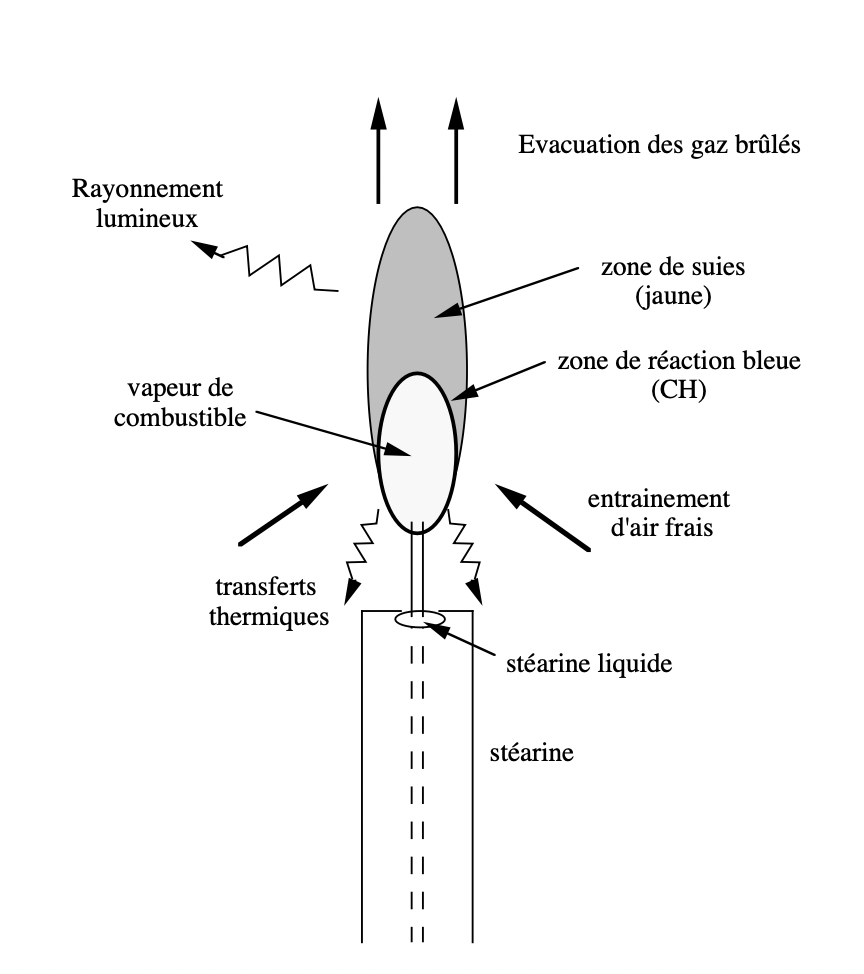
\includegraphics[width=.49\linewidth]{figures/Candle.png}
    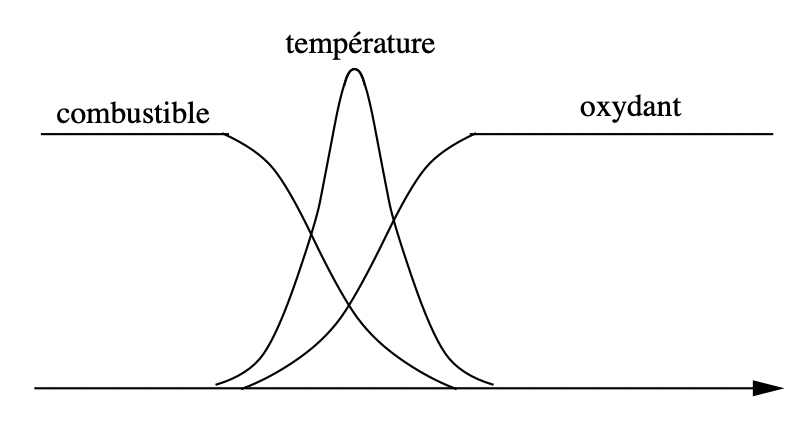
\includegraphics[width=.49\linewidth]{figures/Reaction_Zone.png}
    \caption{Four major combustion phenomena summarized in the example of a candle}
\end{figure}

\pagebreak
Candles can be used as an example to illustrate these four phenomena:
\begin{itemize}
    \item \emph{Chemistry:} Blue reaction zone ($CH^*$ radiation, intermediary chemical reaction).
    \item \emph{Heat transfer:} Soot (unburnt carbon particles) radiation. Liquefaction of stearin at the top of the candle due to conductive heat transfer in the wick and radiation.
    \item \emph{Fluid mechanics:} Natural convection carries fresh air towards the base of the flame and ensures the evacuation of burnt gases.
    \vspace{4pt}
    \\
    \underline{\textbf{\small Remark:}} In microgravity, the candle can go out due to the accumulation of burnt gases near the flame.
\end{itemize}
\pagebreak
\section{Basics}
\subsection{Some definitions}
\subsubsection{Combustion reactions}
Air composition:
\[Air = O_2 + \beta_1N_2 + \beta_2Ar\]
\begin{center}
(with $\beta_1 = 3.717$ and $\beta_2 = 0.047$)\\    
\end{center}
\noindent
Argon presence is usually ignored, we therefore say that:
\[\mathbf{Air = O_2 + 3.764\,N_2}\]
which is equivalent to 21\% oxygen and 79\% nitrogen.\\
Combustion reactions often involve hydrocarbon fuels ($C_nH_m$ where n and m are not necessarily \emph{integers}, especially in mixtures of hydrocarbons, i.e: natural gas). In stoichiometric conditions (enough oxygen to convert all carbon to $CO_2$ and hydrogen to $H_2O$), the balanced chemical equation takes the form:
\[C_nH_m + (n+ \frac{m}{4})(O_2+3.76\,N_2) \rightarrow n\,CO_2 + \frac{m}{2}\,H_2O+3.76(n+\frac{m}{4})\,N_2\]

\subsubsection{State variables, intensivity, and extensivity}

\textbf{State variables} are used to describe combustion processes. \underline{\emph{Temperature}} and \underline{\emph{composition}} describe the state of a mixture at any point in time. \underline{\emph{Pressure}} is an additional state variable that is necessary to fully characterize a reacting mixture, but most combustion applications happen in isobaric conditions so pressure variations are neglected in the textbook.
At the initial state (ambient temperature and no external energy input), the mixture is in \emph{metastable state}. The initial and final state of a reactive mixture is defined by the \textbf{temperature} and \textbf{chemical composition}.
\vspace{4pt}
\\
\underline{\textbf{\small Remark:}} Temperature is however an \textit{intensive} physical quantity from a thermodynamic point-of-view (punctual in space, doesn't take into consideration the dimensions of the system) which is not very convenient. Enthalpy or internal energy are used instead, which are both \textit{intensive properties} (proportional to a characteristic quantity of the system, usually mass or volume).\\
The same can be applied to chemical composition. Mass ($Y_k$) and molar ($X_k$) fractions are used instead:
\begin{itemize}
    \item Mass fraction: \[Y_k = \frac{m_k}{m} = \frac{\rho_k}{\rho}\]
    -- For balanced combustion reactions:
    \[Y_k = \frac{m_k}{m_{tot}} = \frac{\overbrace{n_k}^\textrm{Stoichiometric factor in balanced equation}.\overbrace{M_k}^\textrm{Molar mass of molecule}}{\sum_{k} n_k M_k}\]
    \item Molar fraction: \[X_k = \frac{n_k}{n}\]
    -- For balanced combustion reactions:
    \[X_k = \frac{n_k}{n_{tot}} = \frac{\overbrace{n_k}^\textrm{Stoichiometric factor in balanced equation}}{\sum_{k} n_k}\]
    \item \emph{Another very useful equation:}
    \begin{itemize}
        \item Molar mass of the mixture:
            \[W = \frac{1}{n} \sum n_kW_k = \sum X_k W_k = \frac{1}{\sum \frac{Y_k}{W_k}}\]
    \begin{center}
    (with $\rho_k = W_k C_k$, more details on Ronan's cheat sheet if needed)
    \end{center}
    \end{itemize}
\end{itemize}
\subsubsection{Global variables, equivalence ratio}
In addition to state variables, \textbf{global variables} can also help describe a system (i.e: burner or combustion chamber). \\
One of the most used ones is the \underline{\emph{equivalence ratio}} $\phi$:
\[ \phi = \frac{Y_{fuel}/Y_{oxidizer}}{Y_{fuel}/Y_{oxidizer}}_{st}\]
\begin{center}
    \textit{(can also be written in terms of molar fractions $X_k$)}
\end{center}
It can also be calculated using mixture fractions ($\alpha$):
\[\phi = \frac{\alpha}{\alpha_s}\]
with:
\[\alpha = \frac{\dot{m}_{fuel}}{\dot{m}_{oxidizer}}\]
\[\alpha_s = \frac{nW_C+mW_H}{(n+\frac{m}{4})(W_{O_2}+3.76W_{N_2})}\]
\underline{\emph{Example:}}\\ \\
\textbf{-- Stoichiometry} ($\phi = 1$):
\[C_nH_m + (n+ \frac{m}{4})(O_2+3.76\,N_2) \rightarrow n\,CO_2 + \frac{m}{2}\,H_2O+3.76\,(n+\frac{m}{4})\,N_2\]
\textbf{-- Lean} ($\phi < 1$):
\[\phi\,C_nH_m + (n+ \frac{m}{4})(O_2+3.76\,N_2) \rightarrow \phi\, (n\,CO_2 + \frac{m}{2}\,H_2O)+(n+\frac{m}{4})((1-\phi)O_2+3.76\,N_2)\]
\textbf{-- Rich} ($\phi > 1$):
\[\phi\,C_nH_m + (n+ \frac{m}{4})(O_2+3.76\,N_2) \rightarrow n\,CO_2 + \frac{m}{2}\,H_2O+(\phi-1)C_nH_m+3.76\,(n+\frac{m}{4})\,N_2\]
\begin{center}
\emph{(can contain traces of CO if rich, writing a balance equation can in this case be delicate)}
\end{center}
\pagebreak
\subsection{Thermodynamics and flame temperatures}
\subsubsection{Local thermodynamic equilibrium, thermodynamic systems}
Thermodynamics of reactive flows typically rely on the local thermodynamic equilibrium hypothesis (LTE) -- hypothesis of continuous media (validity criterion: $Kn<<1$). In this case, the intensive and extensive properties are continuous in an arbitrarily small volume dV.
\vspace{8pt}
\\
\underline{\textbf{\small Reminder:}} From Jean Taine's heat transfer book:
\begin{quote}
\emph{
Toute la physique des transferts dans les milieux continus repose sur l'hypothèse de l'équilibre thermodynamique local (E.T.L. ou L.T.E. dans la bibliographie anglo-saxonne) qui correspond à une situation de déséquilibre faible : pendant un intervalle de temps dt et dans un élément de volume dV arbitrairement petits, mais à l'échelle macroscopique, le système matériel est infiniment voisin d'un état d'équilibre tangent, caractérisé par un ensemble de valeurs des grandeurs physiques intensives et extensives.\\ Concrètement l'hypothèse de l'E.T.L. signifie qu'il est possible de définir, à chaque instant t, en tout point r, les variables physiques usuelles en particulier la température T(\textbf{r},t). Elle revient à admettre que les degrés internes du système matériel sont thermalisés (distribution de Maxwell-Boltzmann des populations sur les niveaux d'énergie). Un critère simple de validité des conditions de l'E.T.L. dans un élément de volume dV macroscopiquement petit est que le libre parcours moyen (l.p.m.) des porteurs responsables de la thermalisation soit petit par rapport à une dimension L de cet élément (Kn= l.p.m./L, nombre de Knudsen, petit devant 1.)
}
\end{quote}

\subsubsection{Some important definitions}
\textbf{Thermodynamic systems} --  Some types of thermodynamic systems are described in the following table:

\begin{figure}[ht]
    \centering
    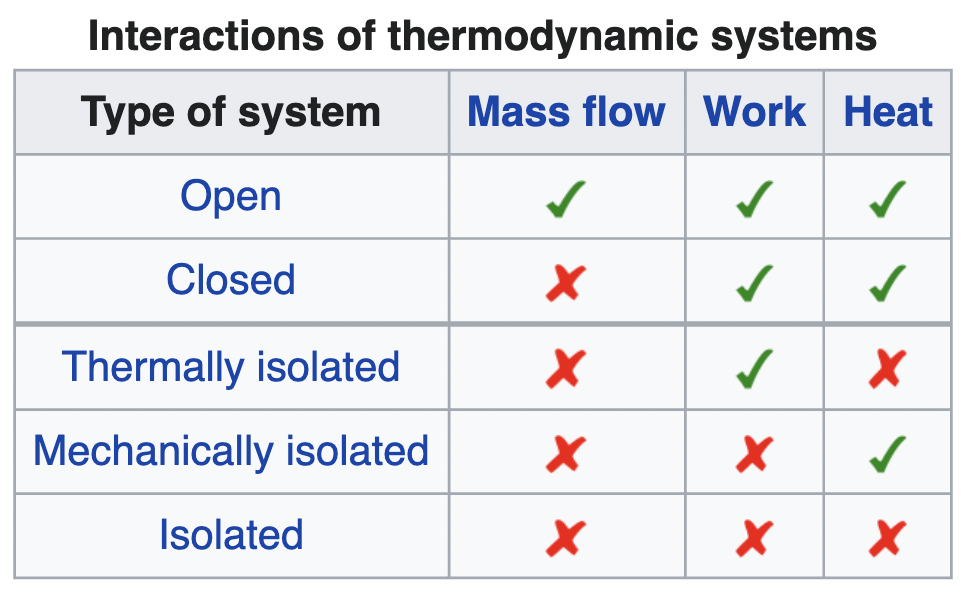
\includegraphics[width=.5\linewidth]{figures/interactions.png}
\end{figure}
\noindent
\textbf{Open system} -- Can exchange mass, work, heat with the exterior.\\
\textbf{Closed system} -- Fixed mass, no exchange of mass with the exterior.\\
\textbf{Isolated system} -- No exchange of mass, heat, or work with the exterior.\\
\emph{Adiabatic \underline{process}} -- No exchange of heat or mass with the exterior (only work).\\

\textbf{Enthalpy (H) } (J) -- Enthalpy is a \textbf{state function} (def: a function that quantitatively describes an equilibrium state of a thermodynamic system, independently of the path / a function of \textbf{state variables} at a certain thermodynamic equilibrium state.)\\
It is defined as the sum of the internal energy and the product of pressure and volume:
\[H = \underbrace{U}_\textrm{Internal energy} + \underbrace{pV}_\textrm{Work}\]

\begin{theo}{First Law of Thermodynamics}-
-- Variant of the energy balance (\emph{"energy can't be created or destroyed, it can only be transformed"}).\\
-- For a \textbf{closed} system:
\[\underbrace{\delta Q}_\textrm{infinitesimal amount of heat} = \underbrace{dU}_\textrm{internal state energy} + \underbrace{\delta W}_\textrm{infinitesimal amount of work}\]
\emph{The work term is sometimes neglected since it's small compared to internal energy.}\\
\emph{Usually, pressure variations can be neglected: $\delta W=pdV$}
\end{theo}
\vspace{10pt}
\textbf{Entropy (S)} ($J.K^{-1}$) -- Entropy is a state function commonly referred to as the degree of disorder in a system. It is also the measurement of the probability of each energy configuration, the number of possibilities (Boltzman's equation), spread of energy (low spread = low entropy, high spread = high entropy).\\
It does not depend on the size of the system, it depends on the probability of spread. Higher entropy is \emph{almost always} more likely, and the chances of entropy decreasing are extremely low especially at the scale of the objects we use.
For a thermodynamic process:
\[adiabatic\,+\,reversible \rightarrow isentropic\]
The opposite, however, is not always true.\\
\begin{theo}{Second Law of Thermodynamics}-
-- Multiple statements (Carnot, Clausius, Kelvin...)\\
-- For a \textbf{closed} system:\\
There exists a quantity S, called the entropy, which has the property that for an infinitesimal process in a \textbf{closed} system, the following inequality always holds (only equal if the process is reversible).
\[ dS \geq \frac{\delta Q}{T} \]
\emph{The equality holds if the process is reversible.}\\
\emph{If the process is adiabatic, $\delta Q = 0$ which gives $dS \geq 0$.}
\end{theo}
\vspace{10pt}
\noindent{
\underline{\textbf{Some interesting relations:}}\\ \\
-- Enthalpy differential using Maxwell equations:
\[dH = dU + d(pV) = dU + pdV + Vdp\]
-- For a \textbf{closed} system, and neglecting pressure variations: (\underline{\emph{Combustion reactions}})
\[dH = \delta Q\]
-- For a \textbf{closed} system, reversible process, and neglecting pressure variations: (\underline{\emph{Not}} valid for combustion // irreversible)
\[dH = TdS+pdV\]
for ideal gases:
\[dH = C_p dT\]
with $C_p$ the heat capacity at constant pressure.
}
\\ \\
\indent 
\textbf{Heat of reaction ($H_r$)} ($J.mol^{-1}$) -- Also referred to as the \textbf{enthalpy of reaction}. It is the change of energy or heat content associated with a reaction at a specified temperature, \underline{where each of the reactants and products is in an appropriate \textbf{standard state}} (def: for each state, a reference state exists -- for gases, it's the ideal gas state at atmospheric pressure). \\
-- \emph{Important:} The heats of reaction should be at the same temperature.\\
Heat of reaction is a \textbf{state function}. The total enthalpy of a system cannot be measured directly, we measure the \textbf{enthalpy change} ($\Delta H$) instead.\\
The heat of reaction can be calculated using three different methods (more details in Appendix A):
\begin{enumerate}
    \item \underline{\textbf{Enthalpy of formation ($\Delta H_f$).}}
    \item \textbf{Bond enthalpies ($\Delta H$, $\Delta H_B$).}
    \item \textbf{Hess's law:} adding up enthalpies of reactions of different chemical reactions to obtain the enthalpy of reaction of the desired reaction (pretty much like summing a bunch of algebraic equations to cancel out some parameters and only keep the final equation -- valid since it's a state function).
\end{enumerate}
For the rest, we will stick to the first definition (\textbf{enthalpy of formation}). In general, it can be calculated using the following equation:
\[\Delta H = \sum _{i\,prod} n_i[(H^{\circ}_{T_2}-H^{\circ}_{0})-(H^{\circ}_{T_0}-H^{\circ}_{0})+(\Delta H^{\circ}_f)_{T_0}]_i
- \sum _{j\,react} n_i[(H^{\circ}_{T_1}-H^{\circ}_{0})-(H^{\circ}_{T_0}-H^{\circ}_{0})+(\Delta H^{\circ}_f)_{T_0}]_j\]
By simplifying (\emph{$T'_0$ can be different for each reactor}):
\[\Delta H = \sum _{i\,prod} n_i[H^{\circ}_{T_2}-H^{\circ}_{T_0}+(\Delta H^{\circ}_f)_{T_0}]_i
- \sum _{j\,react} n_i[H^{\circ}_{T_1}-H^{\circ}_{T_0}+(\Delta H^{\circ}_f)_{T_0}]_j\]
Another definition (Centrale textbook), this time for specific enthalpy:
\[\underbrace{h_k (T,P)}_\textrm{Specific enthalpy of species 'k'} = \underbrace{\Delta h^0_{f,k}(T_0,P_0)}_\textrm{Standard state/ reference enthalpy}+\underbrace{\int_{T_0}^{T}C_{p,k}(T')dT}_\textrm{Sensible enthalpy}\]
\[\underbrace{h (T,P)}_\textrm{Total specific enthalpy} = \sum^K_{k=1} h_k(T,P) =\sum^{K}_{k=1}[Y_k\Delta h^0_{f,k}(T_0,P_0)+\int_{T_0}^{T}Y_kC_{p,k}(T')dT']\]
with $T_0$ standard reference temperature ($298 K$), $T_1$ initial temperature of reactants (sometimes $T_1=T_0$), $T_2$ final temperature of products.

\subsubsection{Adiabatic flame temperature}
In adiabatic conditions, the enthalpy is conserved in combustion reactions. We can write the following equations to estimate the adiabatic flame temperature $T_2$:
\[\Delta h = 0\]
\[h_{reactants} = h_{products}\]
\[\sum^{K}_{k=1}[Y_k\Delta h^0_{f,k}(T_0,P_0)+\int_{T_0}^{T_1}Y_kC_{p,k}(T')dT']_{reactants} = \sum^{K}_{k=1}[Y_k\Delta h^0_{f,k}(T_0,P_0)+\int_{T_0}^{T_2}Y_kC_{p,k}(T')dT']_{products}\]\\
\noindent
\emph{\underline{Quick hacks:}}\\ \\
-- Standard enthalpy of formation ($\Delta h_f^0$) of $O_2$, $N_2$, $H_2$, solid $C$ is equal to zero.\\
-- Initial temperature $T_1=T_0=298\,K$: the integral term in the LHS disappears.
\\
-- Three simplifications for the \textbf{heat capacity at constant pressure} ($C_p$):
\begin{enumerate}
    \item $C_p$ independent of temperature.
    \item $C_p$ same for all species.
    \item (1) and (2) combined.
\end{enumerate}
\emph{Example:} Case 3 -- $C_p$ independent of temperature and same for all species.\\
For the following stoichiometric chemical reaction:
\[CH_4+2(O_2+\beta N_2) \rightarrow CO_2 + 2 H_2O +2\beta N_2\]
\[T_2 = \frac{Y_{CH_4}.\Delta h_f^0(CH_4)
- Y_{CO_2}.\Delta h_f^0(CO_2)
- Y_{H_2O}.\Delta h_f^0(H_2O)}
{C_p}+T_0
\]








\pagebreak
\section{Chemical kinetics}
\subsection{Introduction}
Combustion reactions are characterized by the rates at which they happen and reaction conditions. Some of the most important conditions are temperature, pressure, species concentrations (reactants) and the presence (or absence) of catalysts or inhibitors. Understanding the chemical mechanisms of combustion reactions is therefore of utmost importance. Moreover, the analysis of the production or destruction of pollutants, as well as some important phenomena such as ignition or extinction.\\
Combustion reactions can be modelled using \textbf{global reactions}. A general form is:
\[A + \nu B \rightarrow P\]
Such models are commonly used in complex systems where the calculation of the aerodynamic field takes up most of the computation power and where accounting for all detailed chemical mechanisms is virtually impossible. In reality, combustion reactions are the sum of many elementary reactions.
\subsubsection{Molecular collisions, reaction frequency}
Combustion reactions are initiated at high temperatures where the probability of molecular collisions increases. The \textbf{frequency of molecular collisions} (by volume unit) $Z_{AB}$ is defined as:
\[Z_{AB} = N_a^2 [A] [B] \sigma_{AB} v_{AB}\]
with the \textbf{motion molecular velocity} $v_{AB}$ defined as:
\[v_{AB}=\sqrt{\frac{8k_B T}{\pi \mu{AB}}}\]
with: $N_{a}$: Avogadro's constant ($6.022.10^23$ particles), $[A]$: molar concentration (moles per volume unit) of species A, $\sigma_{AB}$: cross section of possible collisions ($\Pi r_{AB}^2=(r_A+r_B)^2$), $k_B$: Bolzmann's constant (gas constant/$N_a$, $1.381.10^{-23}$, in $J.K^{-1}$), $\mu_{AB}$: reduced mass ($\frac{1}{\mu_{AB}}=\frac{1}{m_A}+\frac{1}{m_B}$), T: Temperature.\\
But since not all collisions lead to reactions, two other correcting factors are added to the above stated equation to model the frequency of collisions \textbf{leading to reactions}.
\begin{itemize}
\item \textbf{Steric factor} (p): probability that colliding molecules are "properly oriented".
\item \textbf{Energetic factor} (f): probability that the energy content of colliding molecules is higher than a certain activation energy ($E_a$ in $J.mol^{-1}$). This term corresponds to the exponential factor in the Arrhenius equation:
\[f=e^\frac{E_a}{RT}\]
\end{itemize}
The frequency of molecular collisions \emph{leading to reactions} (by unit volume) is therefore defined as:
\[v = p.f.Z_{AB}\]
or
\[v = k[A][B]\]
where k is a constant that depends on temperature and can easily be determined by identification.
\subsubsection{Rate of reactions, Arrhenius' law}
Arrhenius' postulate defines the \textbf{rate of reaction \underline{constant}} as:
\[k(T) = \underbrace{A.T^\beta}_{pre-exponential factor} \underbrace{e^\frac{E_a}{RT}}_{exponential (energetic) factor}\]
where A, $\beta$, and $E_a$ are empirical and vary from an author to another.\\
The \textbf{reaction rate} can then be calculated using the constant k. For a simple direct (one-way) reaction of the form:
\[\nu'_A A + \nu'_B B \rightarrow \nu''_C C + \nu''_D D\]
the reaction rate of species A is:
\[\frac{d[A]}{dt} = - k \nu'_A [A]^{\nu'_A} [B]^{\nu'_B}\]


\subsection{Spontaneous combustion}
\pagebreak
\section{Premixed flames}
\pagebreak
\section{Diffusion flames}
\pagebreak


\appendix
\section{Entropy and disorder}
\begin{enumerate}
\item \textbf{Enthalpies of chemical reactions}
\noindent    
\begin{itemize}
\[\Delta H = H_f - H_i \]
\item Heat released during a chemical reaction ($\Delta H<0$) or required ($\Delta H>0$) to initiate it.
\item $\Delta H = \Delta U$ ($p \Delta V$ term small compared to $\Delta U$ so it is often omitted).
\item Enthalpy is a state function (independent of path). It depends only on the initial and final states.
\item \textbf{Hess's law:} adding up enthalpies of reactions of different chemical reactions to obtain the enthalpy of reaction of the desired reaction (pretty much like summing a bunch of algebraic equations to cancel out some parameters and only keep the final equation).
\begin{figure}[h]
\centering                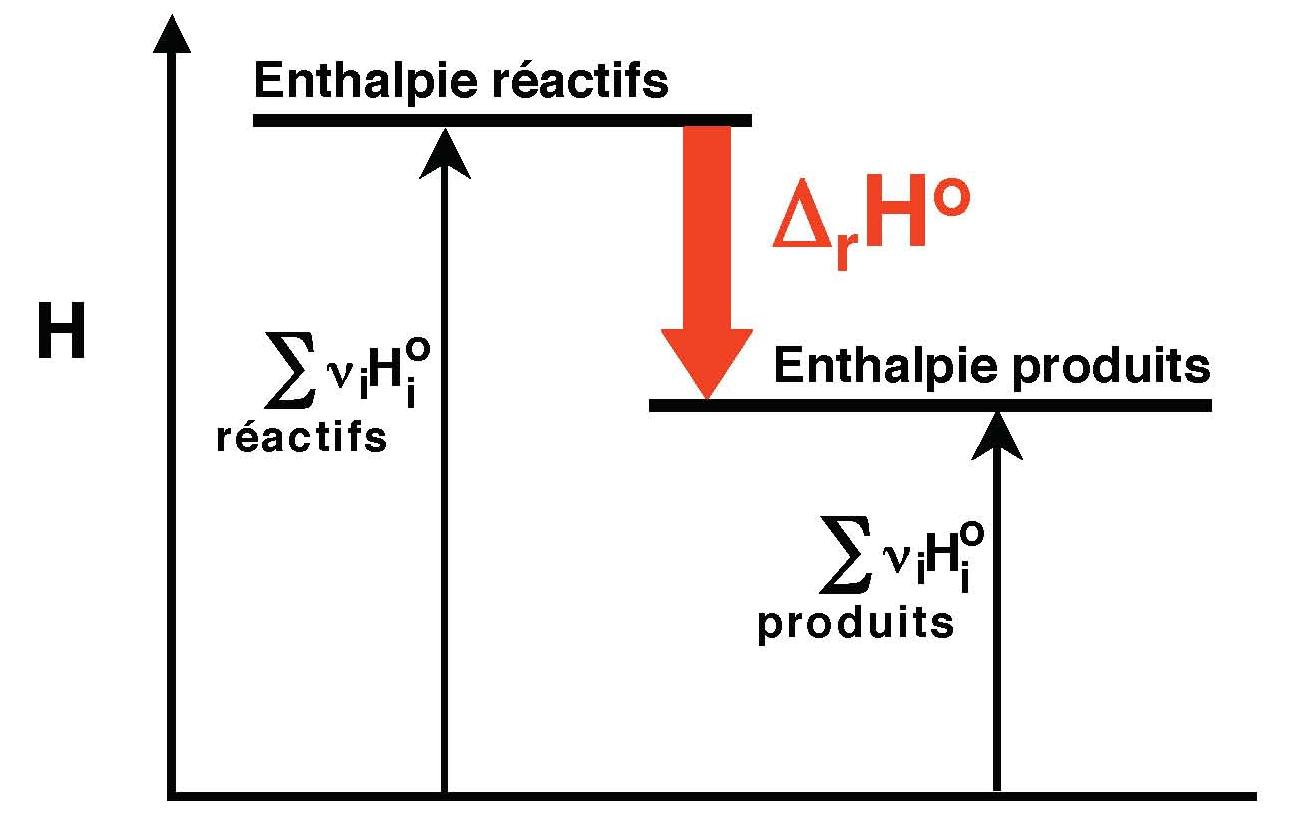
\includegraphics[width=.4\linewidth]{figures/EtatRefEnthalpie.jpeg}
\caption{L'enthalpie de réaction correspond à la différence d'enthalpie entre les produits de la réaction (à droite) et les réactifs (à gauche). Pour calculer cette différence, il est capital de disposer d'une référence commune.}
\end{figure}
\item \textbf{Three way to calculate the heat of reaction:}
\begin{enumerate}
    \item \textbf{Bond enthalpies ($\Delta H$, $\Delta H_B$) :} 
    \[\Delta H_r = \sum \Delta H(bonds \,broken) - \Delta H(bonds\, formed)\]
    \[\Delta H_r = \sum \Delta H(reactants) - \Delta H(products)\]
    
    \item \underline{\textbf{Enthalpy of formation ($\Delta H_f$):}} \emph{(what we typically use in combustion)}
    \[\Delta H_r = \sum \Delta H_f(products) - \Delta H_f(reactants)\]
    \item \textbf{Hess's law.}
\end{enumerate}

        \end{itemize}
    \item \textbf{Spontaneous change and free energy}
        \begin{itemize}
        \item Reaction will proceed in a direction without any external interference to force it to happen.
        \item Endothermic equations are \textbf{more likely} to be non-spontaneous than exothermic reactions. However, endothermic equations \textbf{can be spontaneous} (i.e: melting of a solid $H_2O$ cube).
        \item However, \textbf{enthalpy isn't a measure of spontaneity}, we use instead the \textbf{Gibbs free energy} to assess whether a reaction is spontaneous or not.
        \item \textbf{Gibbs free energy ($\Delta G$) :}
        \[\underbrace{\Delta G}_\textrm{Useful work or free energy} = \Delta H - \underbrace{T \Delta S}_\textrm{Amount of energy that gets "stuck" in molecules (i.e: vib, rot...)}\]
        for constant temperature and pressure.
            \begin{enumerate}
                \item \textbf{$\Delta G < 0$ :} Spontaneous.
                \item \textbf{$\Delta G = 0$ :} Equilibrium (no net change).
                \item \textbf{$\Delta G > 0$ :} Non-spontaneous.
            \end{enumerate}
        \end{itemize}
    \item \textbf{Entropy}
        \begin{itemize}
            \item Measure of disorder of a system.
            \item Change of entropy: are we becoming more ordered or more disordered?
            \item Also a state function (only depends on initial and final state).
            \item \textbf{Entropy of reaction ($\Delta S_r$):}
            \[\Delta S_r^0 = \sum \Delta S^0(products) - \Delta S^0(reactants)\] 
            where $S^0$ is the absolute standard enthalpy.\\
            Important: Multiply S of products or reactants by corresponding stoichiometric coefficient (with S in $kJ.K^{-1}.mol^{-1}$)
            \item S = 0 for the perfect crystal at absolute zero $T=0\,K$ \textbf{(Third law of thermodynamics)}.
            \item Don't confuse \textbf{thermodynamics} (no info on timescales) and \textbf{kinetics} (info about timescales, speed of reactions, etc.)
        \end{itemize}
    \item \textbf{Free energy of formation}
          
        \begin{itemize}
        \item \textbf{Free energy of formation
        ($\Delta G_f$) : } Stability of a compound relative of its elements.
            \[\Delta G^0_f = \Delta H^0_f - T \Delta S^0\]
            ** 0 superscript: standard thermodynamic state (arbitrary reference, typically $P=1\,bar$ and $T=298.15\,K$).
            \begin{enumerate}
                \item \textbf{$\Delta G_r < 0$ :} Stable.
                \item \textbf{$\Delta G_r > 0$ :} Unstable.
            \end{enumerate}
        \end{itemize}    
\end{enumerate}

\end{document}
